\chapter{Tools}

In this section, we focuses on the tools and frameworks used to implement the models and conduct the experiments.

\section{Weights and Biases}

Weights and Biases (W\&B) \cite{wandb} is a machine learning experiment tracking platform that allows users to log and compare the results of different experiments. 
In our research, we used W\&B to track experiments and compare the results of different models.

W\&B provides an intuitive experiment tracking interface that allows users to easily organize and compare results from different runs.
It also provides useful features such as visualization tools, automatic logging of metrics and hyperparameters, and integration with popular machine learning frameworks such as TensorFlow and PyTorch.

We used W\&B to log metrics and hyperparameters such as accuracy, learning rate, batch size, and more. 
This allowed us to easily compare the results of different models and identify which hyperparameters had the most significant impact on performance.

In addition to logging metrics and hyperparameters, W\&B also allowed us to visualize the results in a variety of ways. 
We used the platform's dashboard to plot and compare the different metrics across experiments.

\begin{figure}[H]
  \centering
  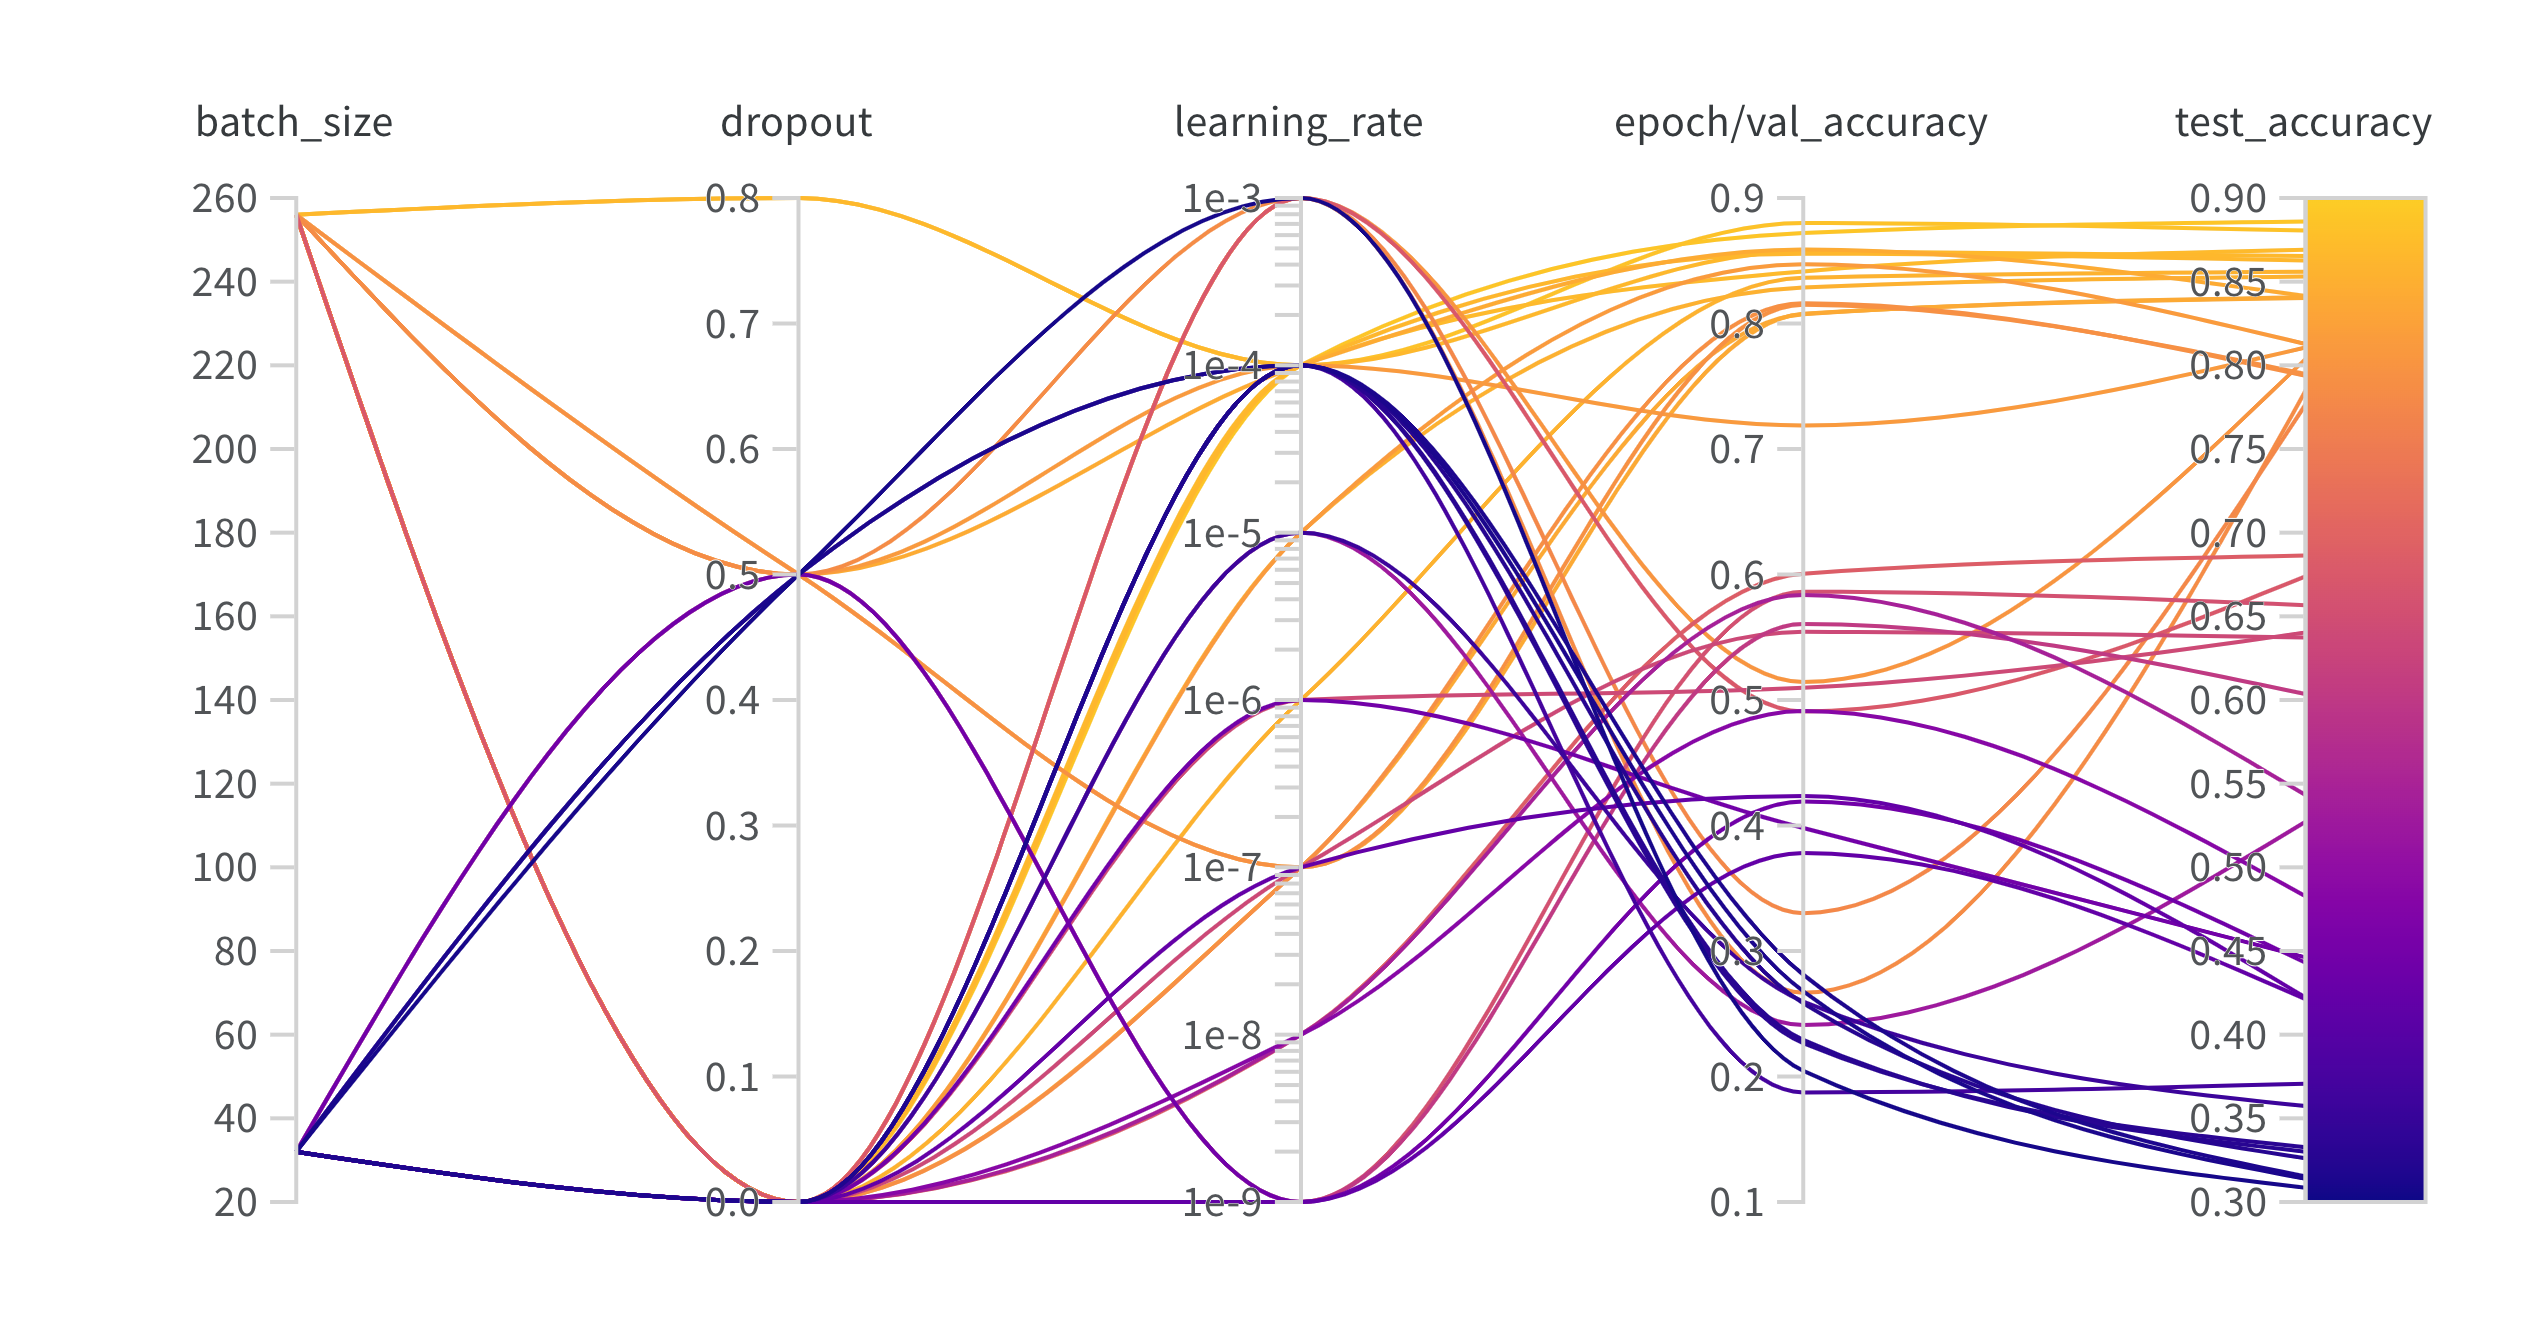
\includegraphics[width=0.4\textwidth]{wandb1}
  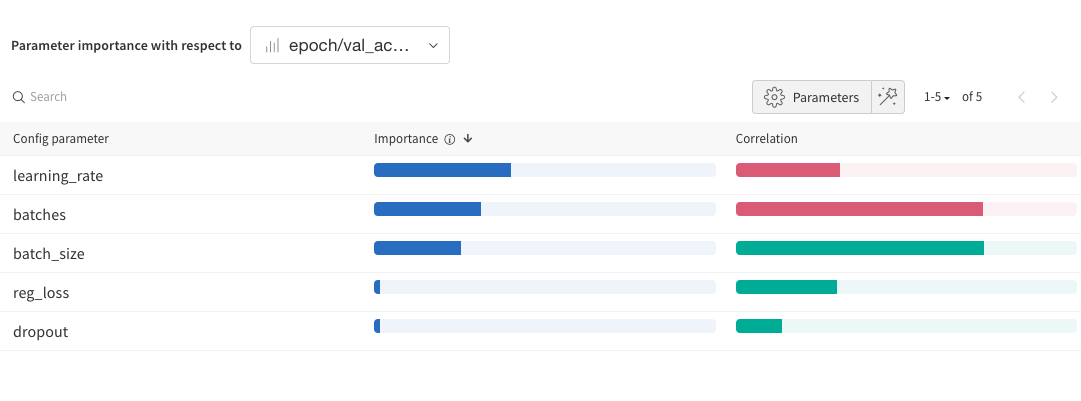
\includegraphics[width=0.4\textwidth]{wandb2}
  \caption{W\&B panels showing parallel coordinates plot of hyperparameters and metrics on the left, and parameter importance plot on the right.}
\end{figure}


To facilitate hyperparameter tuning, W\&B provides a powerful tool called Sweeps.
This feature allows an efficient and automated search of the hyperparameter space, where the user defines a range of values for each hyperparameter and W\&B does the rest.
You can add multiple agents to run the sweeps in parallel, which can significantly reduce the time required to complete the search.
In addition, the results of the sweeps can be easily visualized and compared, providing valuable insight into the impact of different hyperparameters on the performance of the model.

\begin{figure}[H]
\begin{lstlisting}[language=yaml]
method: random
metric:
  goal: maximize
  name: epoch/val_accuracy
parameters:
  G_epoch:
    value: 1
  batch_size:
    value: 32

  # ... more hyper-parameters

  hidden_size:
    value: 128
  learning_rate:
    values:
      - 1e-05
      - 1e-06
      - 1e-07
      - 1e-08
      - 1e-09
program: train.py
\end{lstlisting}
\caption{Example of Sweep configuration}
\end{figure}

Overall, W\&B proved to be an essential tool for our project, allowing us to keep track of the experiments and compare the results of the different models. 
Its intuitive interface and powerful visualization tools made it easy to use and allowed us to quickly gain insight into the performance of the models.


\section{Frameworks}

With the exception of the L-TAE model, which was implemented using PyTorch \cite{NEURIPS2019_9015}, all other models in this study were implemented using TensorFlow \cite{tensorflow2015-whitepaper}.

TensorFlow is a popular and widely used open source machine learning framework developed by Google, which provides an efficient and flexible way to build and train neural networks.

PyTorch, on the other hand, is another popular open-source machine learning framework developed by Facebook that provides dynamic computational graphs and a more python-like way to build and train neural networks, making it particularly suitable for research purposes.

Using both TensorFlow and PyTorch to implement the models was a challenging task, but it provided an opportunity to improve my skills in working with different deep learning frameworks.

